%% Firmware working flow. No tikzlibrary, no siunitx, colours written inline.
\tikzset{every picture/.style={line width=0.75pt}}

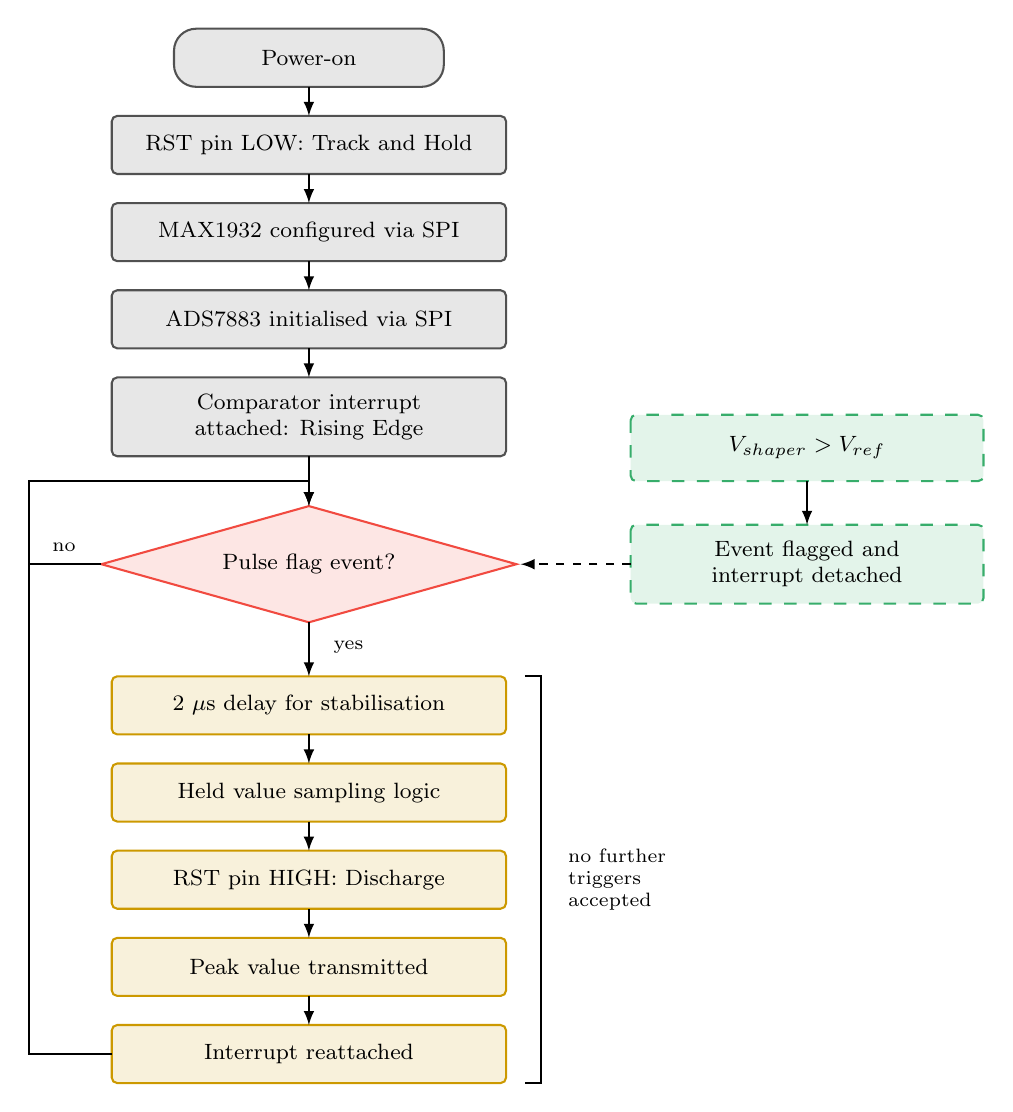
\begin{tikzpicture}[x=0.75pt,y=0.75pt,yscale=-1,xscale=1]

%% ---------------- initialisation (grey) ----------------
\draw [color={rgb, 255:red, 81; green, 81; blue, 81 }, fill={rgb, 255:red, 231; green, 231; blue, 231 }, rounded corners=8pt] (95,4) rectangle (225,32);
\draw [color={rgb, 255:red, 81; green, 81; blue, 81 }, fill={rgb, 255:red, 231; green, 231; blue, 231 }, rounded corners=2pt] (65,46) rectangle (255,74);
\draw [color={rgb, 255:red, 81; green, 81; blue, 81 }, fill={rgb, 255:red, 231; green, 231; blue, 231 }, rounded corners=2pt] (65,88) rectangle (255,116);
\draw [color={rgb, 255:red, 81; green, 81; blue, 81 }, fill={rgb, 255:red, 231; green, 231; blue, 231 }, rounded corners=2pt] (65,130) rectangle (255,158);
\draw [color={rgb, 255:red, 81; green, 81; blue, 81 }, fill={rgb, 255:red, 231; green, 231; blue, 231 }, rounded corners=2pt] (65,172) rectangle (255,210);

\draw [-latex] (160,32) -- (160,46) ;
\draw [-latex] (160,74) -- (160,88) ;
\draw [-latex] (160,116) -- (160,130) ;
\draw [-latex] (160,158) -- (160,172) ;
\draw [-latex] (160,210) -- (160,234) ;

%% ---------------- decision (red) ----------------
\draw [color={rgb, 255:red, 241; green, 74; blue, 64 }, fill={rgb, 255:red, 253; green, 230; blue, 228 }] (60,262) -- (160,234) -- (260,262) -- (160,290) -- cycle ;

%% ---------------- readout chain (yellow) ----------------
\draw [color={rgb, 255:red, 204; green, 153; blue, 0 }, fill={rgb, 255:red, 248; green, 241; blue, 219 }, rounded corners=2pt] (65,316) rectangle (255,344);
\draw [color={rgb, 255:red, 204; green, 153; blue, 0 }, fill={rgb, 255:red, 248; green, 241; blue, 219 }, rounded corners=2pt] (65,358) rectangle (255,386);
\draw [color={rgb, 255:red, 204; green, 153; blue, 0 }, fill={rgb, 255:red, 248; green, 241; blue, 219 }, rounded corners=2pt] (65,400) rectangle (255,428);
\draw [color={rgb, 255:red, 204; green, 153; blue, 0 }, fill={rgb, 255:red, 248; green, 241; blue, 219 }, rounded corners=2pt] (65,442) rectangle (255,470);
\draw [color={rgb, 255:red, 204; green, 153; blue, 0 }, fill={rgb, 255:red, 248; green, 241; blue, 219 }, rounded corners=2pt] (65,484) rectangle (255,512);

\draw [-latex] (160,290) -- (160,316) ;
\draw [-latex] (160,344) -- (160,358) ;
\draw [-latex] (160,386) -- (160,400) ;
\draw [-latex] (160,428) -- (160,442) ;
\draw [-latex] (160,470) -- (160,484) ;

%% return path and idle branch
\draw [-latex] (65,498) -- (25,498) -- (25,222) -- (160,222) -- (160,234) ;
\draw (60,262) -- (25,262) ;

%% ---------------- interrupt (green) ----------------
\draw [color={rgb, 255:red, 55; green, 173; blue, 107 }, fill={rgb, 255:red, 227; green, 244; blue, 234 }, dash pattern={on 4.5pt off 4.5pt}, rounded corners=2pt] (315,190) rectangle (485,222);
\draw [color={rgb, 255:red, 55; green, 173; blue, 107 }, fill={rgb, 255:red, 227; green, 244; blue, 234 }, dash pattern={on 4.5pt off 4.5pt}, rounded corners=2pt] (315,243) rectangle (485,281);

\draw [-latex] (400,222) -- (400,243) ;
\draw [-latex, dash pattern={on 3pt off 3pt}] (315,262) -- (262,262) ;

%% ---------------- interval with no trigger accepted ----------------
\draw (264,316) -- (272,316) -- (272,512) -- (264,512) ;

%% ---------------- text ----------------
\draw (160,18) node [anchor=center, font=\footnotesize, align=center] {Power-on};
\draw (160,60) node [anchor=center, font=\footnotesize, align=center] {RST pin LOW: Track and Hold};
\draw (160,102) node [anchor=center, font=\footnotesize, align=center] {MAX1932 configured via SPI};
\draw (160,144) node [anchor=center, font=\footnotesize, align=center] {ADS7883 initialised via SPI};
\draw (160,191) node [anchor=center, font=\footnotesize, align=center] {Comparator interrupt\\attached: Rising Edge};

\draw (160,262) node [anchor=center, font=\footnotesize, align=center] {Pulse flag event?};

\draw (160,330) node [anchor=center, font=\footnotesize, align=center] {2~$\mu$s delay for stabilisation};
\draw (160,372) node [anchor=center, font=\footnotesize, align=center] {Held value sampling logic};
\draw (160,414) node [anchor=center, font=\footnotesize, align=center] {RST pin HIGH: Discharge};
\draw (160,456) node [anchor=center, font=\footnotesize, align=center] {Peak value transmitted};
\draw (160,498) node [anchor=center, font=\footnotesize, align=center] {Interrupt reattached};

\draw (400,206) node [anchor=center, font=\footnotesize, align=center] {$V_{shaper} > V_{ref}$};
\draw (400,262) node [anchor=center, font=\footnotesize, align=center] {Event flagged and\\interrupt detached};

\draw (167,302) node [anchor=west, font=\scriptsize, align=left] {yes};
\draw (42,254) node [anchor=center, font=\scriptsize, align=center] {no};
\draw (280,414) node [anchor=west, font=\scriptsize, align=left] {no further\\triggers\\accepted};

\end{tikzpicture}